\documentclass[tikz,border=3pt]{standalone}
\usepackage[utf8]{inputenc}
\usepackage[T1]{fontenc}
\usepackage{lmodern}
\renewcommand{\familydefault}{\sfdefault}
\usepackage{sansmath}\sansmath
\usepackage{chemfig}
\usepackage{pgfplots}\pgfplotsset{compat=1.18,/pgf/number format/use comma,/pgf/number format/1000 sep={.}}
\usetikzlibrary{arrows.meta,calc,positioning,decorations.pathmorphing,patterns}
% paleta del sitio
\definecolor{nar}{HTML}{E8680C}\definecolor{narc}{HTML}{FFB35C}\definecolor{hielo}{HTML}{FFF3E8}
\definecolor{tinta}{HTML}{1D1D1F}\definecolor{gris}{HTML}{6E6E73}\definecolor{lila}{HTML}{7C5CF0}
\definecolor{azul}{HTML}{2F6FD6}\definecolor{menta}{HTML}{17A673}\definecolor{coral}{HTML}{E8342A}
\begin{document}
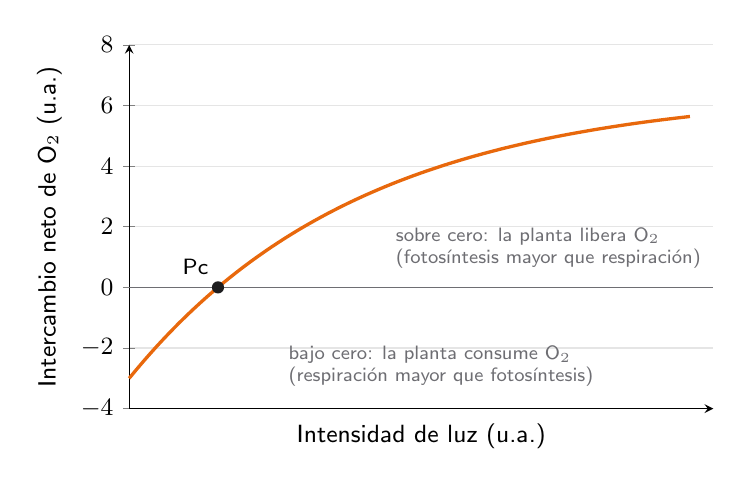
\begin{tikzpicture}[font=\small]
\begin{axis}[width=9cm,height=6.2cm,axis lines=left,xmin=0,xmax=12.5,ymin=-4,ymax=8,xtick=\empty,ytick={-4,-2,0,2,4,6,8},xlabel={Intensidad de luz (u.a.)},ylabel={Intercambio neto de O$_2$ (u.a.)},grid=major,grid style={gray!20},clip=false]
\addplot[gris,thin] coordinates {(0,0)(12.5,0)};
\addplot[nar,very thick,domain=0:12,samples=80] {9.5*(1-exp(-0.2*x))-3};
\fill[tinta] (axis cs:1.9,0) circle (2.2pt);
\node[anchor=south east,font=\footnotesize] at (axis cs:1.9,0.1) {Pc};
\node[font=\scriptsize,text=gris,align=left,anchor=west] at (axis cs:3.2,-2.6) {bajo cero: la planta consume O$_2$\\(respiración mayor que fotosíntesis)};
\node[font=\scriptsize,text=gris,align=left,anchor=west] at (axis cs:5.5,1.3) {sobre cero: la planta libera O$_2$\\(fotosíntesis mayor que respiración)};
\end{axis}
\end{tikzpicture}
\end{document}
